\chapter{Échanges gazeux et transport des sèves chez les plantes}\label{ch:b1:plant-transport}

À la cime d'un séquoia, cent mètres au-dessus du sol, l'eau est tirée
hors de la terre par l'évaporation des \omterm{def:b1:flowering-plant-organization:organs}{feuilles}, le long d'une colonne
de \omterm{def:b1:cell-unit-of-life:cell}{cellules} mortes pas plus large qu'un cheveu, sous une tension qui
romprait un fil d'acier de même section. Il n'y a aucune \omterm{def:b1:membranes-transport:transporters}{pompe}~; l'eau
est hissée par les \omterm{def:b1:water-small-molecules:water}{liaisons hydrogène} mêmes qui la font s'accrocher à
elle-même. Pendant ce temps, dans un second jeu de tubes accolé au
premier, le sucre fabriqué par ces \omterm{def:b1:flowering-plant-organization:organs}{feuilles} s'écoule en sens inverse,
poussé par une pression que les \omterm{def:b1:flowering-plant-organization:organs}{feuilles} engendrent elles-mêmes. Les
deux plomberies d'une plante, le \omterm{def:b1:flowering-plant-organization:tissues}{xylème} et le \omterm{def:b1:plant-transport:phloem}{phloème}, sont mues par
une physique que la plante met en place puis laisse fonctionner. Ce
chapitre décrit les \omterm{def:b1:flowering-plant-organization:tissues}{stomates} par lesquels une \omterm{def:b1:flowering-plant-organization:organs}{feuille} échange de l'eau
contre du dioxyde de carbone, le mécanisme de cohésion--tension qui
hisse la sève, les vaisseaux qui la portent, le flux de masse qui
déplace le sucre, et le compromis entre boire et manger qui gouverne
le tout.

\section{Les stomates~: la porte}

\begin{definition}[Stomate, cellules de garde]\label{def:b1:plant-transport:stoma}
\index{stomate}\index{cellule de garde}
Un \emph{stomate} est un pore de l'épiderme d'une \omterm{def:b1:flowering-plant-organization:organs}{feuille} (ou d'une
\omterm{def:b1:flowering-plant-organization:organs}{tige} verte) bordé par deux \emph{\omterm{def:b1:cell-unit-of-life:cell}{cellules} de garde}, \omterm{def:b1:cell-unit-of-life:cell}{cellules}
réniformes dont les parois sont épaissies du côté du pore et dont les
microfibrilles de \omterm{def:b1:carbohydrates:polysaccharide}{cellulose} les ceinturent comme des cerceaux. Quand
les \omterm{def:b1:cell-unit-of-life:cell}{cellules} de garde absorbent de l'eau et gonflent, les cerceaux les
empêchent de s'élargir et les forcent à s'arquer en s'écartant~: le
pore s'ouvre. Quand elles perdent de l'eau, il se ferme. Une \omterm{def:b1:flowering-plant-organization:organs}{feuille}
porte quelques centaines de \omterm{def:b1:flowering-plant-organization:tissues}{stomates} par millimètre carré, surtout à
sa face inférieure~; ouverts, leurs pores font un ou deux pour cent de
la surface foliaire et presque tous ses échanges gazeux y passent.
\end{definition}

\begin{omfigure}
\begin{tikzpicture}
  \node[anchor=south west, inner sep=0] (img) at (0,0)
    {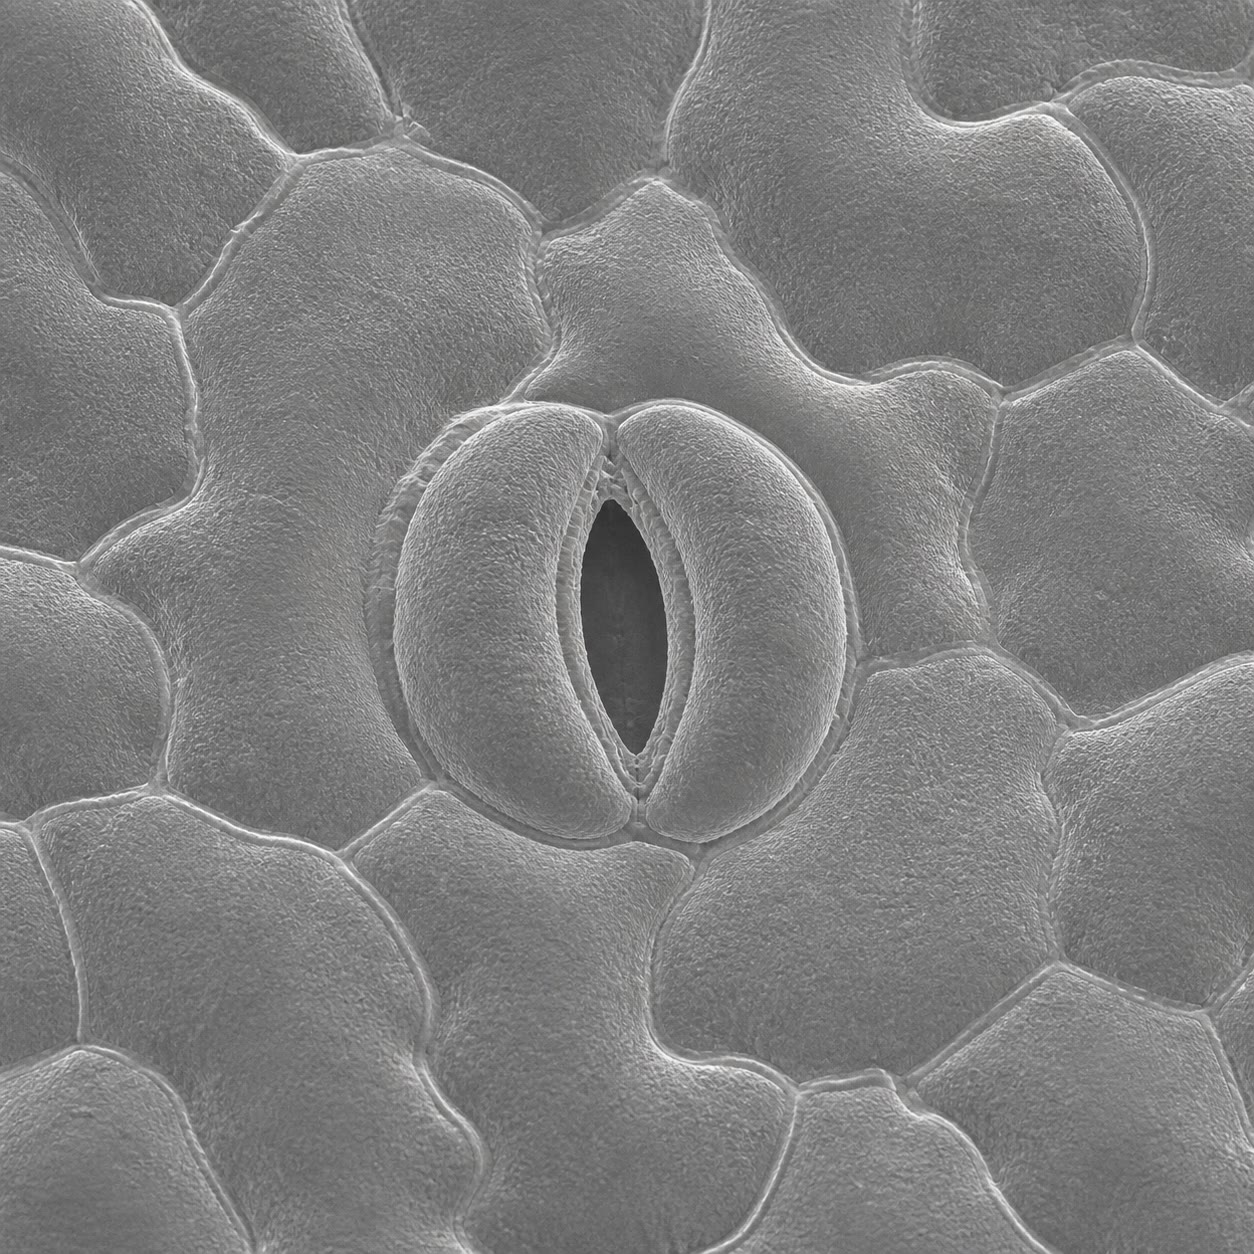
\includegraphics[width=0.4\linewidth]{images/book2/ai/g12-plant-stoma-sem.jpg}};
  \begin{scope}[x={(img.south east)}, y={(img.north west)},
      every node/.style={font=\small}]
    \draw[omDef, thick] (0.50,0.50) -- (0.50,1.08) node[above] {pore};
    \draw[omDef, thick] (0.30,0.55) -- (-0.03,0.70) node[left, align=right] {cellule de garde~:\\ paroi interne épaisse};
    \draw[omDef, thick] (0.80,0.30) -- (1.03,0.20) node[right, align=left] {cellules épidermiques\\ à cuticule};
  \end{scope}
\end{tikzpicture}

{\small Un \omterm{def:b1:plant-transport:stoma}{stomate} vu de l'extérieur~: deux \omterm{def:b1:plant-transport:stoma}{cellules de garde} autour du
pore, dans un épiderme ciré. Le pore s'ouvre quand les \omterm{def:b1:plant-transport:stoma}{cellules de
garde} gonflent.}
\end{omfigure}

\begin{proposition}[Comment un stomate s'ouvre, et quand]\label{prop:b1:plant-transport:opening}
\index{acide abscissique}
Les \omterm{def:b1:plant-transport:stoma}{cellules de garde} ouvrent le pore en expulsant des protons
(\cref{ch:b1:plant-water-minerals}), ce qui fait entrer potassium et
chlorure et produire du malate à l'intérieur~; les solutés abaissent
leur \omterm{def:b1:membranes-transport:osmosis}{potentiel hydrique}, l'eau vient des \omterm{def:b1:cell-unit-of-life:cell}{cellules} voisines, et leur
\omterm{def:b1:eukaryotic-cell:plantcell}{turgescence} monte d'un mégapascal. Inverser les flux d'ions referme le
pore en quelques minutes. Les signaux~: la \emph{lumière} (la lumière
bleue directement sur les \omterm{def:b1:plant-transport:stoma}{cellules de garde}, et la chute du
$\mathrm{CO_2}$ interne quand la photosynthèse démarre) ouvre~; un
\emph{$\mathrm{CO_2}$ interne élevé} ferme~; le \emph{stress hydrique}
ferme, par l'hormone \emph{\omterm{prop:b1:plant-transport:opening}{acide abscissique}}, produite dans les
\omterm{def:b1:flowering-plant-organization:organs}{racines} et les \omterm{def:b1:flowering-plant-organization:organs}{feuilles} qui flétrissent, qui déclenche en minutes la
sortie des ions des \omterm{def:b1:plant-transport:stoma}{cellules de garde}~; l'air sec ferme. La \omterm{def:b1:flowering-plant-organization:organs}{feuille}
ouvre sa porte quand le carbone vaut l'eau et la referme quand l'eau
manque --- et la plupart des plantes le font selon un rythme quotidien,
ouvrant à l'aube et fermant au crépuscule, qui persiste des jours
durant en lumière constante.
\end{proposition}

\begin{omfigure}
\begin{tikzpicture}
\begin{axis}[
  width=0.88\linewidth, height=6.0cm,
  axis x line=bottom, axis y line=left,
  xmin=0, xmax=24, ymin=0, ymax=1.15,
  xlabel={heure de la journée (h)}, ylabel={valeur relative},
  xlabel style={font=\small, at={(axis description cs:0.5,-0.12)}, anchor=north},
  ylabel style={font=\small},
  tick label style={font=\small}, xtick={0,4,8,12,16,20,24}, ytick={0,0.5,1},
  legend style={font=\small, at={(0.5,-0.24)}, anchor=north, draw=none, legend columns=3, /tikz/every even column/.append style={column sep=0.4cm}},
  clip=false,
]
\addplot[very thick, omExo, smooth] coordinates {(0,0.05) (5,0.05) (6,0.3) (7,0.8) (8,1.0) (11,1.0) (12,0.75) (13,0.5) (14,0.55) (16,0.8) (18,0.6) (19,0.2) (20,0.05) (24,0.05)};
\addlegendentry{ouverture stomatique}
\addplot[very thick, omDef, smooth] coordinates {(0,0) (5,0) (6,0.1) (8,0.5) (10,0.85) (12,1.0) (14,0.9) (16,0.6) (18,0.3) (19,0.1) (20,0) (24,0)};
\addlegendentry{transpiration}
\addplot[very thick, omThm, smooth] coordinates {(0,0.2) (5,0.2) (7,0.3) (9,0.55) (11,0.8) (13,1.0) (15,0.95) (17,0.7) (19,0.4) (21,0.25) (24,0.2)};
\addlegendentry{potentiel hydrique foliaire (signe inversé)}
\end{axis}
\end{tikzpicture}

{\small Une journée d'été pour une \omterm{def:b1:flowering-plant-organization:organs}{feuille}. Les \omterm{def:b1:flowering-plant-organization:tissues}{stomates} s'ouvrent à
l'aube, la transpiration monte avec le soleil et la sécheresse de
l'air, et le \omterm{def:b1:membranes-transport:osmosis}{potentiel hydrique} de la \omterm{def:b1:flowering-plant-organization:organs}{feuille} chute à mesure que la
colonne est mise sous tension~; à midi, en air sec, les \omterm{def:b1:flowering-plant-organization:tissues}{stomates} se
referment en partie et la \omterm{def:b1:flowering-plant-organization:organs}{feuille} récupère un peu avant l'après-midi.}
\end{omfigure}

\section{Hisser l'eau~: cohésion et tension}

\begin{theorem}[Le mécanisme de cohésion--tension]\label{thm:b1:plant-transport:cohesiontension}
\index{cohesion-tension@théorie de la cohésion--tension}\index{transpiration}
L'eau monte dans le \omterm{def:b1:flowering-plant-organization:tissues}{xylème} parce qu'elle est \emph{tirée} d'en haut,
non poussée d'en bas. L'évaporation depuis les parois humides des
\omterm{def:b1:cell-unit-of-life:cell}{cellules} du mésophylle vers les lacunes (\emph{transpiration}) attire
l'eau des pores fins de la paroi en ménisques courbes, dont la tension
superficielle met sous tension l'eau qui les suit~; la tension est
transmise, par les colonnes d'eau continues du \omterm{def:b1:flowering-plant-organization:tissues}{xylème} que la cohésion
maintient (les \omterm{def:b1:water-small-molecules:water}{liaisons hydrogène} du
\cref{ch:b1:water-small-molecules}), jusqu'au bas de la \omterm{def:b1:flowering-plant-organization:organs}{tige} et dans
les \omterm{def:b1:flowering-plant-organization:organs}{racines}, et hisse l'eau du sol. Retenir une colonne de hauteur $h$
contre la pesanteur exige une tension $\rho g h$ --- \qty{1}{MPa} par
centaine de mètres --- plus ce qu'il faut pour vaincre le frottement de
l'écoulement, à peu près autant~; les colonnes d'un grand arbre sont à
\qtyrange{-2}{-3}{MPa}, bien en deçà de la résistance à la traction de
l'eau dans un tube fin.
\end{theorem}
\begin{proof}[Faits expérimentaux]
Dixon et Joly (1894) montrèrent que l'eau d'un tube de verre scellé
supporte des tensions de plusieurs mégapascals sans rompre, et qu'un
rameau feuillu qui transpire, scellé à un tube d'eau plongeant dans du
mercure, soulève le mercure plus haut que ne le pourrait la pression
atmosphérique. La \emph{chambre à pression} de Scholander (1965) mesure
la tension directement~: une \omterm{def:b1:flowering-plant-organization:organs}{feuille} coupée est scellée dans une
chambre, son pétiole dépassant, et la pression de gaz qui ramène tout
juste la sève à la surface de coupe égale la tension que subissait la
sève --- \qtyrange{0.5}{1}{MPa} dans une culture bien arrosée à midi,
\qtyrange{2}{4}{MPa} dans un arbuste du désert ou la cime d'un grand
arbre. Un dendromètre montre le tronc d'un arbre rétrécir le jour, la
tension comprimant les vaisseaux, et gonfler la nuit~; un thermomètre
dans le bois montre la sève circuler le plus vite quand la
transpiration est maximale, et s'arrêter la nuit. Aucune \omterm{def:b1:cell-unit-of-life:cell}{cellule}
vivante n'est requise~: une \omterm{def:b1:flowering-plant-organization:organs}{tige} tuée par un poison ou par la chaleur
conduit encore.
\end{proof}

\begin{omfigure}
\begin{tikzpicture}[font=\footnotesize, >=Stealth, line cap=round]
  % leaf at top, stem, root in soil; water potentials
  \draw[thick, omExo!70!black, fill=omExo!25] (0,7.0) .. controls (1.4,7.8) and (2.6,7.6) .. (3.0,7.0) .. controls (2.6,6.4) and (1.4,6.2) .. (0,7.0);
  \node[font=\scriptsize] at (1.5,7.0) {feuille, $\Psi = \qty{-1.5}{MPa}$};
  \draw[line width=6pt, omDef!35] (1.5,6.3) -- (1.5,1.6);
  \draw[very thick, omDef!70!black] (1.38,6.3) -- (1.38,1.6) (1.62,6.3) -- (1.62,1.6);
  \node[font=\scriptsize, anchor=west, align=left] at (1.75,4.0) {xylème~: colonne d'eau continue\\ sous tension, $\Psi = \qty{-1.0}{MPa}$ à mi-hauteur};
  \fill[pattern=north east lines, pattern color=omProp!60] (-1.0,0) rectangle (4.0,1.6);
  \draw[thick, omDef!60!black] (1.5,1.6) -- (1.5,0.6) (1.5,1.3) -- (0.6,0.4) (1.5,1.0) -- (2.4,0.3);
  \node[font=\scriptsize, anchor=west] at (2.7,1.1) {racine, $\Psi = \qty{-0.5}{MPa}$};
  \node[font=\scriptsize, anchor=west] at (2.7,0.5) {sol, $\Psi = \qty{-0.2}{MPa}$};
  % evaporation arrows out of leaf
  \foreach \x in {0.6,1.5,2.4} { \draw[->, thick, omThm] (\x,7.55) -- (\x,8.3); }
  \node[anchor=south, omThm] at (1.5,8.35) {transpiration vers un air à $\Psi = \qty{-95}{MPa}$};
  % upward flow arrow
  \draw[->, very thick, omDef!70!black] (-0.6,1.8) -- (-0.6,6.4) node[midway, left, align=right] {sève tirée\\ vers le haut};
  \node[anchor=north, align=center, gray] at (1.5,-0.3) {$\Psi$ baisse à chaque étape du sol à l'air~: le gradient est fixé par l'évaporation au sommet,\\ et la cohésion de l'eau transmet la traction jusqu'aux racines};
\end{tikzpicture}

{\small Cohésion--tension. L'évaporation au niveau de la \omterm{def:b1:flowering-plant-organization:organs}{feuille} y
abaisse le \omterm{def:b1:membranes-transport:osmosis}{potentiel hydrique}~; la tension est transmise le long de
colonnes d'eau ininterrompues dans le \omterm{def:b1:flowering-plant-organization:tissues}{xylème} et tire l'eau du sol.
L'arbre ne fournit aucun travail~: le soleil le fournit.}
\end{omfigure}

\begin{definition}[Conduits du xylème, cavitation]\label{def:b1:plant-transport:xylem}
\index{vaisseau du xyleme@vaisseau du xylème}\index{cavitation}
L'eau circule dans les \emph{\omterm{def:b1:flowering-plant-organization:tissues}{trachéides}} et les \emph{vaisseaux} du
\omterm{def:b1:flowering-plant-organization:tissues}{xylème} (\cref{ch:b1:flowering-plant-organization})~: des \omterm{def:b1:cell-unit-of-life:cell}{cellules}
mortes vidées de leur contenu, aux parois lignifiées épaissies en
anneaux et en spirales qui les empêchent de s'affaisser sous la tension
interne, jointes bout à bout par des perforations (vaisseaux) ou par
des ponctuations de leurs parois latérales (\omterm{def:b1:flowering-plant-organization:tissues}{trachéides}). Un vaisseau
peut être large de \qtyrange{20}{300}{\micro m} et long de quelques
centimètres à quelques mètres~: les tubes larges transportent bien
davantage (le débit dans un tube croît comme la puissance quatrième du
rayon) mais sont plus vulnérables à la \emph{cavitation} --- la
formation soudaine d'une bulle de gaz dans l'eau sous tension, qui vide
le conduit et le met hors service. Les ponctuations entre conduits
empêchent les bulles de se propager~; le gel et la sécheresse causent
tous deux la cavitation, et les vaisseaux d'un arbre sont en partie
remplis à nouveau par la \omterm{prop:b1:plant-water-minerals:rootpressure}{poussée racinaire} au printemps, ou remplacés
par du bois neuf chaque année.
\end{definition}

\begin{omfigure}
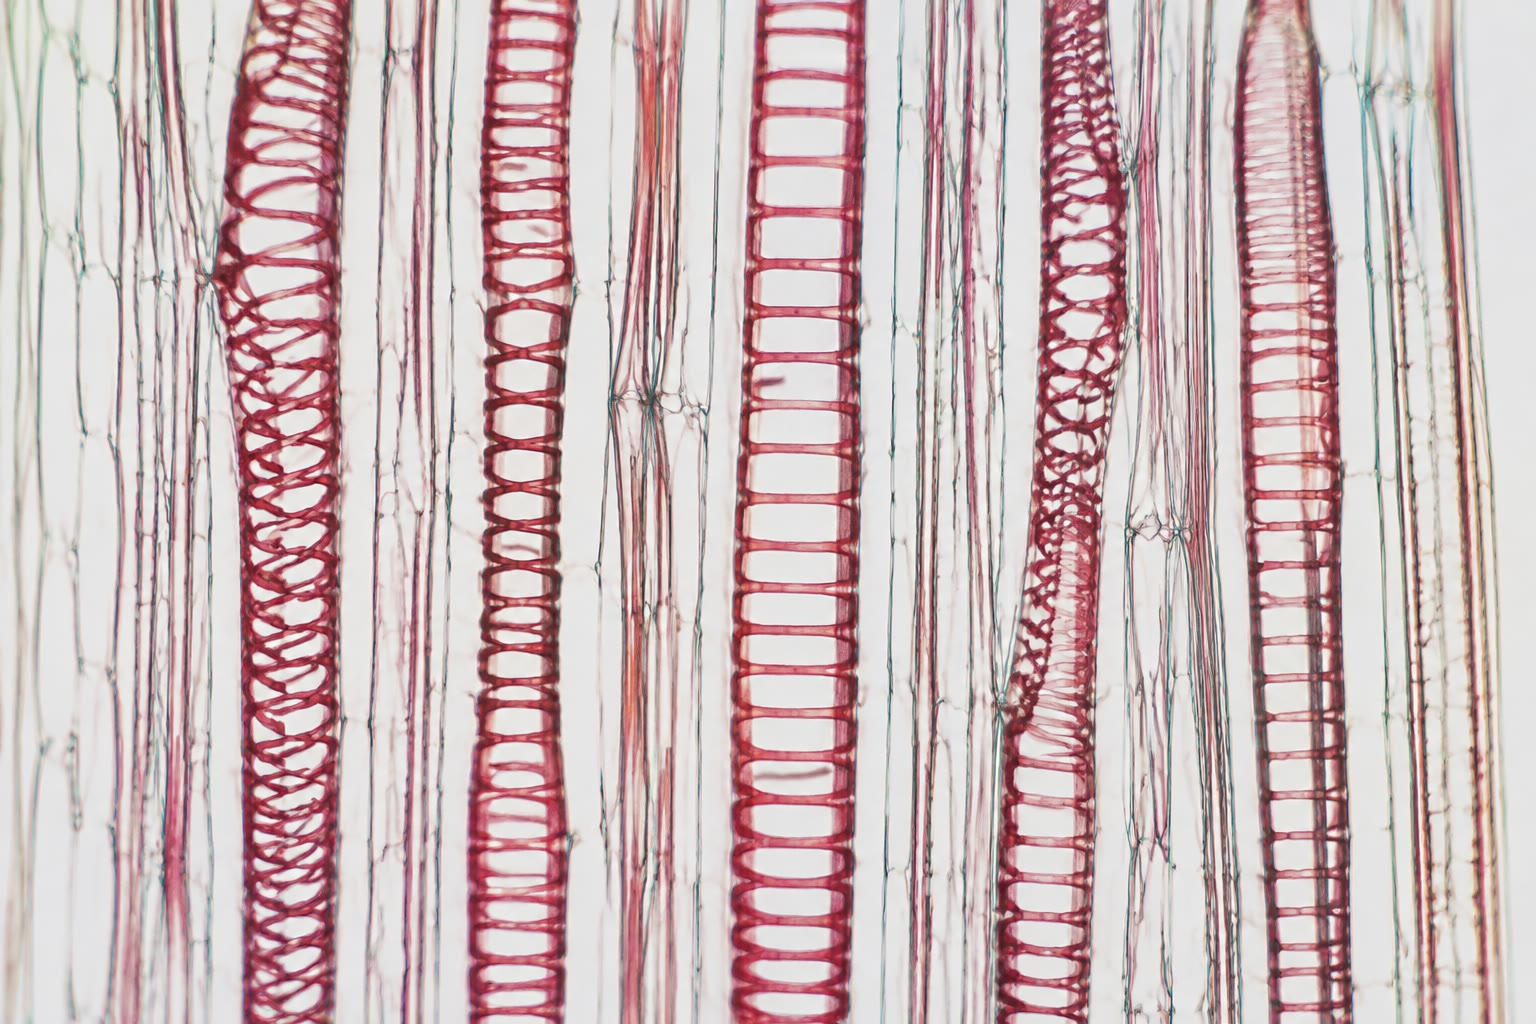
\includegraphics[width=0.52\linewidth]{images/book3/ai/b3-24-xylem-vessels.jpg}

{\small Des vaisseaux du \omterm{def:b1:flowering-plant-organization:tissues}{xylème} en coupe longitudinale~: des tubes creux
dont les parois sont renforcées d'anneaux et de spirales de lignine
contre la tension de la sève qu'ils portent.}
\end{omfigure}

\begin{omfigure}
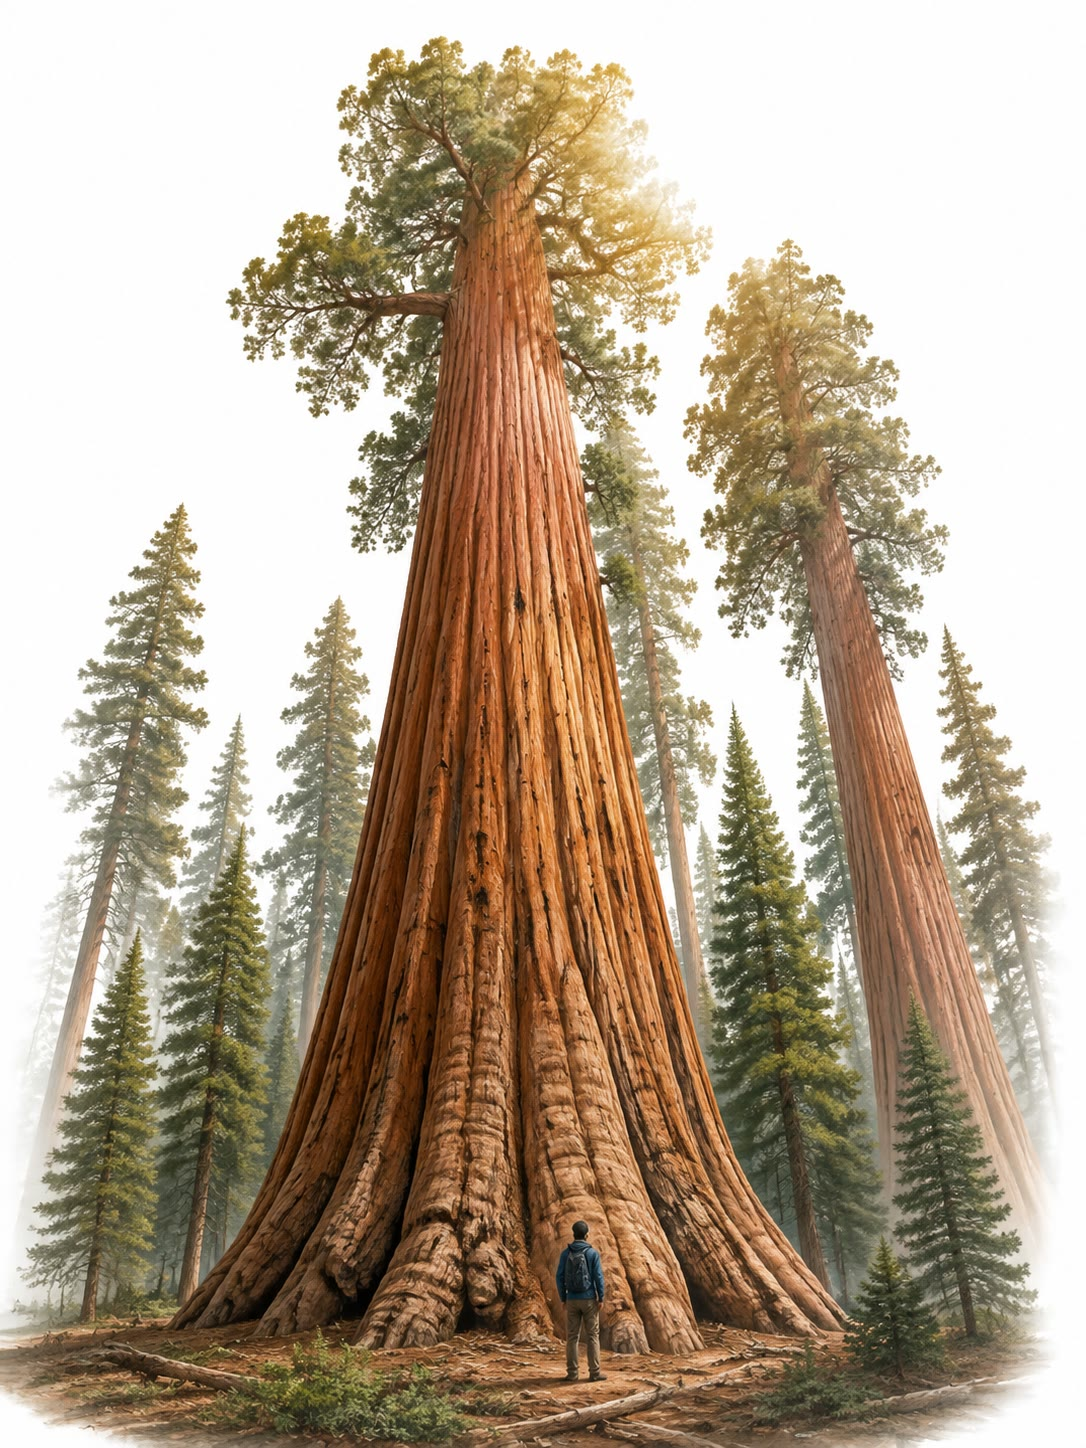
\includegraphics[width=0.36\linewidth]{images/book3/ai/b3-24-sequoia.jpg}

{\small Des séquoias géants. La sève atteint leur cime, cent mètres
plus haut, tirée par l'évaporation des \omterm{def:b1:flowering-plant-organization:organs}{feuilles} à travers des colonnes
d'eau sous une tension de deux mégapascals ou plus.}
\end{omfigure}

\begin{example}[La cime de l'arbre]\label{ex:b1:plant-transport:top}
À \qty{100}{m}, le poids de la colonne exige à lui seul \qty{1}{MPa} de
tension~; le frottement dans les vaisseaux en ajoute autant le jour, si
bien que le \omterm{def:b1:flowering-plant-organization:tissues}{xylème} de la cime est proche de \qty{-2}{MPa} et que les
\omterm{def:b1:cell-unit-of-life:cell}{cellules} foliaires, pour lui prendre de l'eau, sont plus basses
encore~: leurs \omterm{def:b1:flowering-plant-organization:tissues}{stomates} doivent se fermer plus tôt dans la journée et
leur photosynthèse est plus lente que celle d'une branche basse, et les
\omterm{def:b1:flowering-plant-organization:organs}{feuilles} du sommet sont petites et épaisses. La hauteur des arbres les
plus élevés, quelque \qty{120}{m}, est probablement fixée par là~:
au-dessus, les \omterm{def:b1:flowering-plant-organization:organs}{feuilles} ne peuvent tenir la tension sans caviter un
après-midi sec.
\end{example}

\section{Déplacer le sucre~: le flux de masse}

\begin{definition}[Phloème, tubes criblés, source et puits]\label{def:b1:plant-transport:phloem}
\index{phloeme@phloème}\index{tube crible@tube criblé}\index{source}\index{puits}
Le sucre circule dans le \emph{phloème}, dans des \emph{\omterm{def:b1:flowering-plant-organization:tissues}{tubes
criblés}}~: des files de \omterm{def:b1:cell-unit-of-life:cell}{cellules} vivantes qui ont perdu leur noyau et
la plupart de leurs \omterm{def:b1:cell-unit-of-life:prokeuk}{organites} mais gardent leurs membranes, jointes
bout à bout par des \emph{cribles} perforés, chacune assistée d'une
\emph{\omterm{def:b1:cell-unit-of-life:cell}{cellule} compagne} qui lui fournit \omterm{def:b1:proteins:peptide}{protéines} et \omterm{def:b1:water-small-molecules:atp}{ATP}. La sève
contient \qtyrange{10}{30}{\%} de saccharose, avec des \omterm{def:b1:proteins:aminoacid}{acides aminés},
des ions et des molécules de signalisation, et elle va des
\emph{sources} --- \omterm{def:b1:flowering-plant-organization:organs}{feuilles} qui photosynthétisent, ou \omterm{def:b1:mammal-organization:organ}{organes} de
réserve que l'on vide --- vers les \emph{puits} --- apex en croissance,
\omterm{def:b1:flowering-plant-organization:organs}{racines}, fruits, graines, \omterm{def:b1:mammal-organization:organ}{organes} de réserve que l'on remplit --- à
\qtyrange{0.5}{1}{m/h}, dans n'importe quel sens, et dans des sens
différents selon les tubes.
\end{definition}

\begin{theorem}[Le flux de masse]\label{thm:b1:plant-transport:pressureflow}
\index{mecanisme de flux de masse@mécanisme de flux de masse}
La sève élaborée se déplace en masse, sous une différence de pression
hydrostatique entre la source et le \omterm{def:b1:plant-transport:phloem}{puits} (Münch, 1930). À la source,
les \omterm{def:b1:cell-unit-of-life:cell}{cellules} compagnes \emph{chargent} le saccharose dans les \omterm{def:b1:flowering-plant-organization:tissues}{tubes
criblés} contre son gradient (par symport de protons, depuis
l'\omterm{def:b1:plant-water-minerals:pathways}{apoplasme}, ou par les \omterm{def:b1:eukaryotic-cell:plantcell}{plasmodesmes})~; le \omterm{def:b1:membranes-transport:osmosis}{potentiel hydrique} du tube
chute, l'eau vient du \omterm{def:b1:flowering-plant-organization:tissues}{xylème} voisin, et la \omterm{def:b1:eukaryotic-cell:plantcell}{turgescence} monte à
\qty{1}{MPa} ou plus. Au \omterm{def:b1:plant-transport:phloem}{puits}, le saccharose est \emph{déchargé} puis
consommé ou stocké, le \omterm{def:b1:membranes-transport:osmosis}{potentiel hydrique} remonte, l'eau sort, et la
\omterm{def:b1:eukaryotic-cell:plantcell}{turgescence} est faible. Entre les deux, la sève descend le gradient de
pression à travers les cribles, emportant tout ce qui y est dissous. La
plante ne dépense d'énergie qu'aux deux bouts~; l'écoulement lui-même
est passif.
\end{theorem}
\begin{proof}[Faits expérimentaux]
Un puceron qui se nourrit sur une \omterm{def:b1:flowering-plant-organization:organs}{tige} enfonce son stylet dans un seul
\omterm{def:b1:plant-transport:phloem}{tube criblé}~; coupez le puceron et le stylet, laissé en place, exsude
de la sève pendant des heures sous la pression du tube lui-même --- de
la sève élaborée pure, dont on peut mesurer la concentration en
saccharose et le débit, et dont la pression, mesurée au manomètre sur
le stylet, vaut environ \qty{1}{MPa} près d'une source et moins vers le
\omterm{def:b1:plant-transport:phloem}{puits}. Du $\mathrm{^{14}CO_2}$ marqué donné à une \omterm{def:b1:flowering-plant-organization:organs}{feuille} apparaît dans
le \omterm{def:b1:plant-transport:phloem}{phloème} de la \omterm{def:b1:flowering-plant-organization:organs}{tige} en quelques minutes et se déplace à la vitesse
que prédit l'écoulement du stylet~; refroidir un tronçon de \omterm{def:b1:flowering-plant-organization:organs}{tige}, ce
qui ralentit les \omterm{def:b1:cell-unit-of-life:cell}{cellules} vivantes mais n'affecte guère un écoulement
mû par la pression, ne ralentit le transport que très peu~; empoisonner
le chargement de la \omterm{def:b1:flowering-plant-organization:organs}{feuille} source l'arrête.
\end{proof}

\begin{omfigure}
\begin{tikzpicture}[font=\footnotesize, >=Stealth, line cap=round]
  % xylem and phloem tubes side by side
  \draw[line width=8pt, omDef!25] (1.0,0.3) -- (1.0,5.7); \node[anchor=south, omDef!70!black] at (1.0,5.8) {xylème};
  \draw[line width=8pt, omExo!25] (3.6,0.3) -- (3.6,5.7); \node[anchor=south, omExo!70!black] at (3.6,5.8) {phloème (tube criblé)};
  % source at top
  \node[draw, thick, rounded corners=4pt, fill=omExo!15, align=center, minimum width=26mm] (src) at (7.2,5.0) {source~: feuille\\ saccharose chargé};
  \node[draw, thick, rounded corners=4pt, fill=omProp!15, align=center, minimum width=26mm] (snk) at (7.2,1.0) {puits~: racine, fruit\\ saccharose déchargé};
  \draw[->, thick, omExo!70!black] (src.west) -- (3.9,5.0) node[midway, above, font=\scriptsize] {entrée du sucre};
  \draw[->, thick, omProp!80!black] (3.3,1.0) -- (snk.west) node[midway, above, font=\scriptsize] {sortie du sucre};
  % water in from xylem at top, out to xylem at bottom
  \draw[->, thick, omDef!70!black] (1.3,4.6) -- (3.3,4.6) node[midway, below, font=\scriptsize] {l'eau suit};
  \draw[->, thick, omDef!70!black] (3.3,1.5) -- (1.3,1.5) node[midway, below, font=\scriptsize] {l'eau revient};
  % flow arrows
  \draw[->, very thick, omExo!70!black] (3.6,4.2) -- (3.6,2.0) node[midway, right, align=left, font=\scriptsize] {flux de masse suivant le\\ gradient de pression};
  \draw[->, very thick, omDef!70!black] (1.0,2.0) -- (1.0,4.2) node[midway, left, align=right, font=\scriptsize] {courant de\\ transpiration (tension)};
  \node[anchor=west, font=\scriptsize] at (3.9,5.5) {$\Psi_p \approx \qty{+1.0}{MPa}$};
  \node[anchor=west, font=\scriptsize] at (3.9,0.5) {$\Psi_p \approx \qty{+0.3}{MPa}$};
\end{tikzpicture}

{\small Le flux de masse. Charger le saccharose à la source y attire
l'eau du \omterm{def:b1:flowering-plant-organization:tissues}{xylème} et élève la pression~; le décharger au \omterm{def:b1:plant-transport:phloem}{puits} laisse
l'eau sortir et l'abaisse~; la sève s'écoule entre les deux, et l'eau
revient par le \omterm{def:b1:flowering-plant-organization:tissues}{xylème}.}
\end{omfigure}

\begin{omfigure}
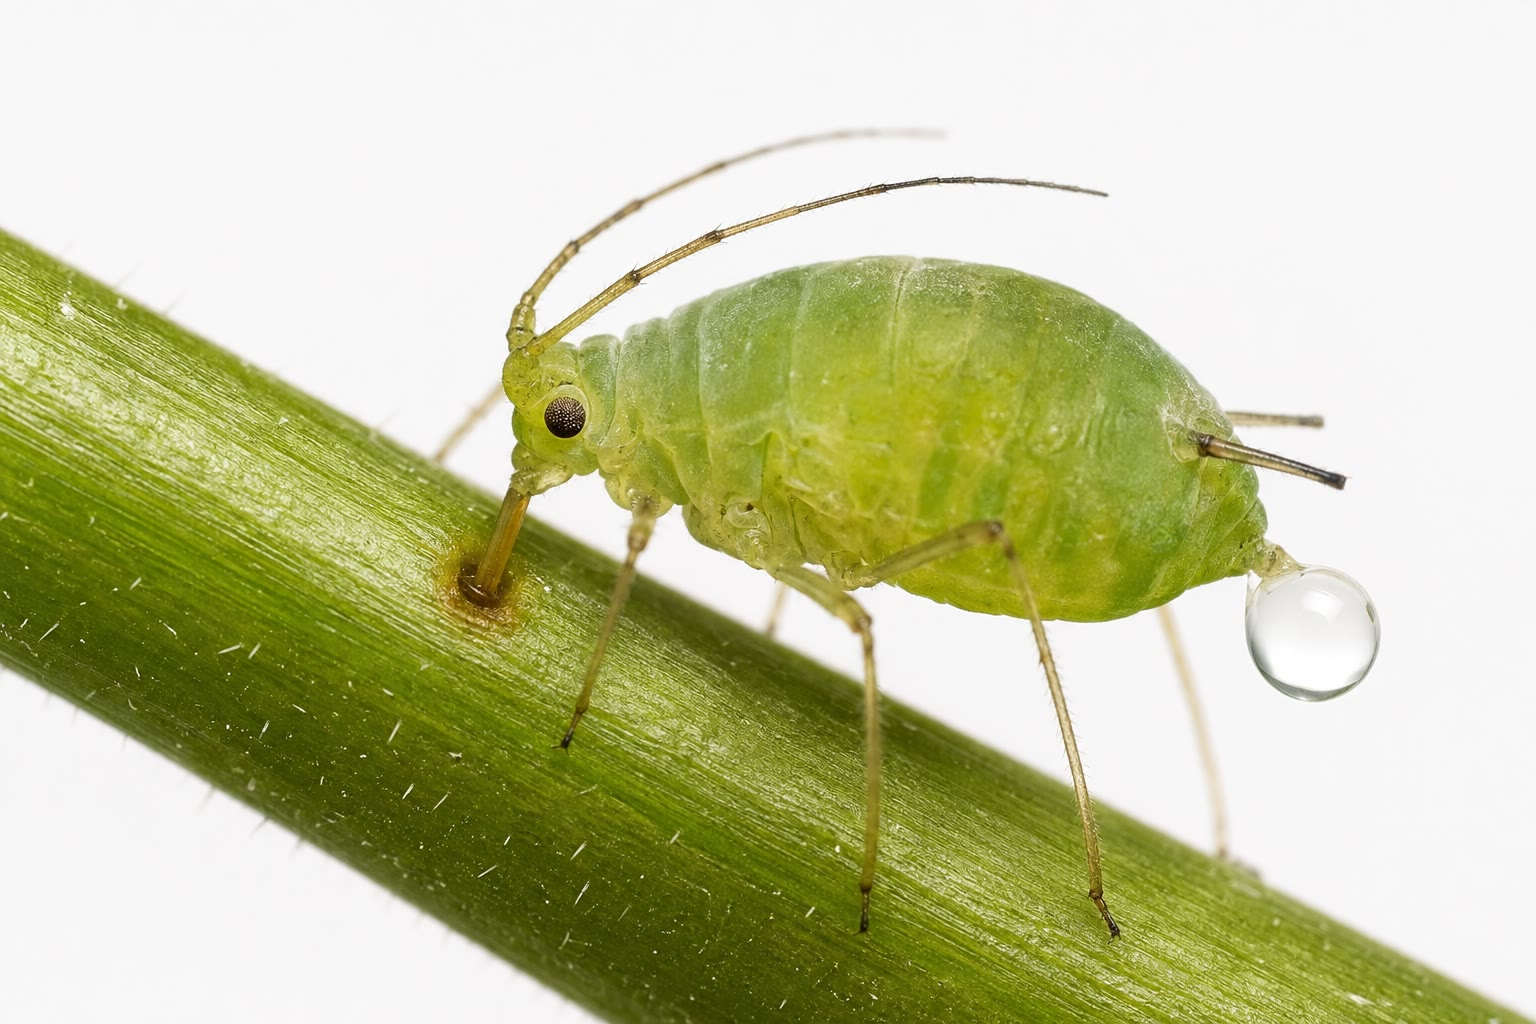
\includegraphics[width=0.5\linewidth]{images/book3/ai/b3-24-aphid-feeding.jpg}

{\small Un puceron se nourrissant sur une \omterm{def:b1:flowering-plant-organization:organs}{tige}~: son stylet, plus fin
qu'un cheveu, est dans un seul \omterm{def:b1:plant-transport:phloem}{tube criblé}, et la pression du \omterm{def:b1:plant-transport:phloem}{phloème}
pousse la sève dans l'insecte --- si bien que le surplus en ressort en
miellat. Sectionné, le stylet devient le robinet du physiologiste.}
\end{omfigure}

\begin{method}[Lire une expérience de translocation]\label{met:b1:plant-transport:translocation}
\begin{enumerate}
  \item Donner à une \omterm{def:b1:flowering-plant-organization:organs}{feuille} du $\mathrm{CO_2}$ marqué~; prélever la
        \omterm{def:b1:flowering-plant-organization:organs}{tige} au-dessus et au-dessous à intervalles~: la position du
        marqueur en fonction du temps donne le sens et la vitesse de
        l'écoulement.
  \item Anneler la \omterm{def:b1:flowering-plant-organization:organs}{tige} (ôter un anneau d'écorce, qui porte le
        \omterm{def:b1:plant-transport:phloem}{phloème}, en laissant le \omterm{def:b1:flowering-plant-organization:tissues}{xylème})~: le sucre s'accumule au-dessus
        de l'anneau et les \omterm{def:b1:flowering-plant-organization:organs}{racines} meurent de faim en dessous --- c'est
        le \omterm{def:b1:plant-transport:phloem}{phloème}, non le \omterm{def:b1:flowering-plant-organization:tissues}{xylème}, qui le porte~; l'arbre meurt en une
        saison.
  \item Recueillir la sève de stylets de pucerons sectionnés à deux
        hauteurs~: la chute du saccharose et de la pression entre eux
        est le gradient qui entraîne l'écoulement.
  \item Changer les \omterm{def:b1:plant-transport:phloem}{puits}~: ôtez les fruits, et le marqueur va aux
        \omterm{def:b1:flowering-plant-organization:organs}{racines}~; ombrez la \omterm{def:b1:flowering-plant-organization:organs}{feuille}, et elle devient elle-même un \omterm{def:b1:plant-transport:phloem}{puits}.
        Le schéma de l'écoulement est celui de la demande.
\end{enumerate}
\end{method}

\begin{example}[Une pomme de terre en deux saisons]\label{ex:b1:plant-transport:potato}
En été, les \omterm{def:b1:flowering-plant-organization:organs}{feuilles} sont les sources et les tubercules souterrains les
\omterm{def:b1:plant-transport:phloem}{puits}~: le saccharose descend, est déchargé, converti en \omterm{def:b1:carbohydrates:polysaccharide}{amidon}, et les
tubercules grossissent. Au printemps, le tubercule germe~: son \omterm{def:b1:carbohydrates:polysaccharide}{amidon}
est reconverti en saccharose, chargé dans le \omterm{def:b1:plant-transport:phloem}{phloème}, et monte vers la
pousse en croissance --- le même tube, le sens inverse, parce que la
source et le \omterm{def:b1:plant-transport:phloem}{puits} ont échangé leurs rôles.
\end{example}

\section{Le compromis}

\begin{proposition}[L'efficience d'utilisation de l'eau]\label{prop:b1:plant-transport:wue}
\index{efficience d'utilisation de l'eau}
Tout \omterm{def:b1:plant-transport:stoma}{stomate} qui laisse entrer du dioxyde de carbone perd de l'eau, et
l'échange est inégal~: l'intérieur de la \omterm{def:b1:flowering-plant-organization:organs}{feuille} est saturé de vapeur et
l'air du dehors est sec, tandis que le $\mathrm{CO_2}$ est à
\qty{0.04}{\%} au dehors et plus bas au dedans, de sorte que le
gradient sortant de l'eau vaut des centaines de fois le gradient
entrant du dioxyde de carbone. Une \omterm{def:b1:flowering-plant-organization:organs}{feuille} en C3 perd
\qtyrange{200}{500}{} molécules d'eau par $\mathrm{CO_2}$ fixé~; une
\omterm{def:b1:flowering-plant-organization:organs}{feuille} en C4, qui concentre le $\mathrm{CO_2}$ et garde ses \omterm{def:b1:flowering-plant-organization:tissues}{stomates}
plus étroits, \qtyrange{100}{200}{}~; une \omterm{def:b1:photosynthesis:c4cam}{plante CAM}, qui n'ouvre que la
nuit, \qtyrange{20}{50}{} (\cref{ch:b1:photosynthesis}).
L'\emph{\omterm{prop:b1:plant-transport:wue}{efficience d'utilisation de l'eau}} est le carbone gagné par eau
perdue, et son amélioration --- fermeture à midi, \omterm{def:b1:flowering-plant-organization:tissues}{stomates} enfoncés et
\omterm{def:b1:flowering-plant-organization:tissues}{cuticules} épaisses, voies C4 et CAM --- est la part que la plante prend
au marché conclu avec une atmosphère sèche.
\end{proposition}

\begin{example}[Le marché en chiffres]\label{ex:b1:plant-transport:bargain}
Un pied de maïs qui transpire un litre et demi par jour fixe quelque
\qty{10}{g} de dioxyde de carbone~: \qty{80}{mol} d'eau pour
\qty{0.23}{mol} de $\mathrm{CO_2}$, trois cent cinquante pour un. Un
champ de blé transpire en une saison cinq cents tonnes d'eau par
hectare pour faire huit tonnes de grain~; l'eau est le prix du carbone,
et dans la plupart des champs du monde c'est ce prix qui limite la
récolte.
\end{example}

\section{Exercices}

\begin{exercise}[$\star$]\label{exo:b1:plant-transport:1}
Expliquer comment la forme et les parois des \omterm{def:b1:plant-transport:stoma}{cellules de garde}
transforment une hausse de \omterm{def:b1:eukaryotic-cell:plantcell}{turgescence} en un pore ouvert.
\end{exercise}

\begin{exercise}[$\star$]\label{exo:b1:plant-transport:2}
Énoncer le mécanisme de cohésion--tension en trois phrases~: d'où vient
la force, ce qui la transmet, ce qu'elle fait à la \omterm{def:b1:flowering-plant-organization:organs}{racine}.
\end{exercise}

\begin{exercise}[$\star$]\label{exo:b1:plant-transport:3}
À partir de la figure de la journée, dire à quelle heure la
transpiration est maximale, quand le \omterm{def:b1:membranes-transport:osmosis}{potentiel hydrique} de la \omterm{def:b1:flowering-plant-organization:organs}{feuille}
atteint son minimum, et pourquoi les \omterm{def:b1:flowering-plant-organization:tissues}{stomates} se referment en partie à
midi.
\end{exercise}

\begin{exercise}[$\star$]\label{exo:b1:plant-transport:4}
Définir source et \omterm{def:b1:plant-transport:phloem}{puits}, et dire ce qui se passe à chacun dans le
\omterm{thm:b1:plant-transport:pressureflow}{mécanisme de flux de masse}.
\end{exercise}

\begin{exercise}[$\star\star$]\label{exo:b1:plant-transport:5}
Calculer la tension nécessaire pour retenir une colonne d'eau haute de
\qty{30}{m} ($\rho g h$), et le total si le frottement la double. Quel
doit être au moins le \omterm{def:b1:membranes-transport:osmosis}{potentiel hydrique} des \omterm{def:b1:flowering-plant-organization:organs}{feuilles} à cette hauteur~?
\end{exercise}

\begin{exercise}[$\star\star$]\label{exo:b1:plant-transport:6}
Le débit dans un tube varie comme $r^4$. Comparer le débit d'un seul
vaisseau de \qty{100}{\micro m} de rayon à celui du nombre de
\omterm{def:b1:flowering-plant-organization:tissues}{trachéides} de \qty{10}{\micro m} qui offre la même section totale.
Pourquoi les plantes gardent-elles les étroites~?
\end{exercise}

\begin{exercise}[$\star\star$]\label{exo:b1:plant-transport:7}
Une sève élaborée à \qty{20}{\%} de saccharose (\qty{0.6}{mol/L}) a un
\omterm{def:b1:membranes-transport:osmosis}{potentiel osmotique} d'environ \qty{-1.5}{MPa}. À côté d'un \omterm{def:b1:flowering-plant-organization:tissues}{xylème} à
\qty{-0.5}{MPa}, quelle \omterm{def:b1:eukaryotic-cell:plantcell}{turgescence} le \omterm{def:b1:plant-transport:phloem}{tube criblé} atteint-il à
l'équilibre~? À un \omterm{def:b1:plant-transport:phloem}{puits} où la sève est à \qty{5}{\%} de saccharose
($\Psi_s = \qty{-0.4}{MPa}$) à côté du même \omterm{def:b1:flowering-plant-organization:tissues}{xylème}, quelle \omterm{def:b1:eukaryotic-cell:plantcell}{turgescence}~?
Quelle différence de pression entraîne l'écoulement~?
\end{exercise}

\begin{exercise}[$\star\star$]\label{exo:b1:plant-transport:8}
Un stylet de puceron exsude \qty{1}{\micro L} par heure de sève à
\qty{20}{\%} de saccharose. Si le \omterm{def:b1:plant-transport:phloem}{tube criblé} a un rayon de
\qty{10}{\micro m}, calculer la vitesse de la sève et le sucre livré
par heure.
\end{exercise}

\begin{exercise}[$\star\star$]\label{exo:b1:plant-transport:9}
Expliquer pourquoi anneler un arbre le tue en une saison, alors que
ses \omterm{def:b1:flowering-plant-organization:organs}{feuilles} restent vertes des semaines après la coupe de l'anneau.
\end{exercise}

\begin{exercise}[$\star\star\star$]\label{exo:b1:plant-transport:10}
Les lacunes d'une \omterm{def:b1:flowering-plant-organization:organs}{feuille} sont saturées à \qty{25}{\celsius}
(\qty{23}{g/m^3} de vapeur)~; l'air extérieur en contient
\qty{9}{g/m^3}. Le $\mathrm{CO_2}$ est à \qty{0.72}{g/m^3} dehors et
\qty{0.45}{g/m^3} dedans. Les deux gaz diffusent par les mêmes pores,
l'eau diffusant 1,6 fois plus vite que le $\mathrm{CO_2}$. Calculer le
rapport de l'eau perdue au $\mathrm{CO_2}$ gagné, en masse et en
molécules.
\end{exercise}

\begin{exercise}[$\star\star\star$]\label{exo:b1:plant-transport:11}
Un après-midi chaud et sec, un vaisseau cavite. Décrire ce qui advient
de la colonne d'eau, de la tension dans les vaisseaux voisins et de la
\omterm{def:b1:flowering-plant-organization:organs}{feuille} qu'il alimentait~; expliquer comment les ponctuations limitent
les dégâts et comment la plante récupère la nuit ou au printemps.
\end{exercise}

\begin{exercise}[$\star\star\star$]\label{exo:b1:plant-transport:12}
«~Un arbre est une mèche entre le sol et le ciel, avec un tuyau à sucre
qui court en sens inverse.~» Discuter en un paragraphe~: ce que porte
chaque système, ce qui l'entraîne, où la plante dépense de l'énergie et
où elle n'en dépense pas.
\end{exercise}

\section{Problème~: le séquoia}

\begin{problem}[{Problème du week-end --- un arbre de cent mètres un
jour d'été~: la tension à sa cime, la vitesse de la sève, l'eau qu'il
déplace, le sucre qu'il envoie vers le bas et le carbone qu'il achète,
jusqu'à la tension du xylème à la cime}]
\label{pb:b1:plant-transport:1}
Un séquoia haut de \qty{100}{m} porte une cime de \qty{2000}{m^2} de
\omterm{def:b1:flowering-plant-organization:organs}{feuilles}. Un jour d'été, il transpire \qty{600}{L} d'eau en
\qty{12}{h} à travers un aubier de section \qty{0.5}{m^2}, dont
\qty{20}{\%} est du lumen conducteur. Eau~: $\rho = \qty{1000}{kg/m^3}$, $g =
\qty{9.8}{m/s^2}$, \qty{18}{g/mol}. Le frottement le long du tronc
coûte autant de tension que la pesanteur. \omterm{def:b1:membranes-transport:osmosis}{Potentiel hydrique} du sol
\qty{-0.1}{MPa}. La cime fixe \qty{4}{\micro mol} de $\mathrm{CO_2}$
par mètre carré de \omterm{def:b1:flowering-plant-organization:organs}{feuille} et par seconde pendant \qty{12}{h}~; le
saccharose fait \qty{342}{g/mol} et porte douze carbones~; la sève
élaborée contient \qty{15}{\%} de saccharose en masse (masse volumique
\qty{1.06}{g/mL}) et s'écoule à \qty{0.6}{m/h}.

\medskip
\noindent\textbf{Partie I --- La tension.}
\begin{enumerate}
  \item Calculer la tension nécessaire pour soutenir la colonne contre
        la pesanteur.
  \item Ajouter le frottement~: quelle est la tension du \omterm{def:b1:flowering-plant-organization:tissues}{xylème} à la
        cime~?
  \item Calculer le \omterm{def:b1:membranes-transport:osmosis}{potentiel hydrique} du \omterm{def:b1:flowering-plant-organization:tissues}{xylème} à la cime, en prenant
        $\Psi_s = 0$ pour la sève.
  \item Quel doit être le \omterm{def:b1:membranes-transport:osmosis}{potentiel hydrique} des \omterm{def:b1:cell-unit-of-life:cell}{cellules} foliaires à
        la cime pour que l'eau y entre~? Si leur $\Psi_s = \qty{-2.5}{MPa}$,
        quelle \omterm{def:b1:eukaryotic-cell:plantcell}{turgescence} ont-elles~?
  \item Comparer avec une \omterm{def:b1:flowering-plant-organization:organs}{feuille} à \qty{10}{m} sur le même arbre ($\Psi_s =
        \qty{-1.5}{MPa}$).
  \item L'eau dans des tubes fins supporte environ \qty{-30}{MPa}~;
        pourquoi l'arbre ne pousse-t-il pas simplement jusqu'à
        \qty{1000}{m}~?
\end{enumerate}

\medskip
\noindent\textbf{Partie II --- L'écoulement.}
\begin{enumerate}[resume]
  \item Calculer le débit de transpiration en litres par heure et en
        mètres cubes par seconde.
  \item Calculer la section conductrice de l'aubier.
  \item Calculer la vitesse moyenne de la sève.
  \item Calculer la masse d'eau contenue dans le lumen conducteur du
        tronc (sur ses \qty{100}{m}).
  \item Combien de temps une molécule d'eau met-elle pour aller de la
        \omterm{def:b1:flowering-plant-organization:organs}{racine} à la cime à cette vitesse~?
  \item Calculer la transpiration par mètre carré de \omterm{def:b1:flowering-plant-organization:organs}{feuille} et par
        heure, en grammes, et par seconde en millimoles.
  \item La sève descend un gradient de potentiel allant de \qty{-0.1}{}
        au sol jusqu'à la valeur de la cime trouvée à la question 3,
        sur \qty{100}{m}. Quel est le gradient en mégapascals par
        mètre~? Comment se compare-t-il à la seule part
        gravitationnelle~?
\end{enumerate}

\medskip
\noindent\textbf{Partie III --- Le sucre.}
\begin{enumerate}[resume]
  \item Calculer le $\mathrm{CO_2}$ fixé par la cime et par jour, en
        moles.
  \item Calculer le saccharose correspondant, en moles et en
        kilogrammes.
  \item La moitié est respirée dans la cime~; le reste descend par le
        \omterm{def:b1:plant-transport:phloem}{phloème}. Calculer la masse de saccharose transloquée par jour
        et la masse de sève qui la porte.
  \item Calculer le volume de sève et, à \qty{0.6}{m/h}, la section de
        \omterm{def:b1:flowering-plant-organization:tissues}{tubes criblés} nécessaire pour la porter en \qty{24}{h}.
  \item Calculer le temps que met le saccharose pour aller de la cime
        à la \omterm{def:b1:flowering-plant-organization:organs}{racine}.
  \item Calculer le rapport d'utilisation de l'eau~: moles d'eau
        transpirées par mole de $\mathrm{CO_2}$ fixée.
\end{enumerate}

\medskip
\noindent\textbf{Partie IV --- Les compromis.}
\begin{enumerate}[resume]
  \item Le \omterm{def:b1:membranes-transport:osmosis}{potentiel hydrique} de la sève élaborée à la cime, avec
        $\Psi_s = \qty{-1.2}{MPa}$ et une \omterm{def:b1:eukaryotic-cell:plantcell}{turgescence} de \qty{1.0}{MPa}~:
        le calculer et le comparer à celui du \omterm{def:b1:flowering-plant-organization:tissues}{xylème} au même endroit.
        Dans quel sens l'eau passe-t-elle entre les deux, et est-ce
        compatible avec le chargement~?
  \item À la \omterm{def:b1:flowering-plant-organization:organs}{racine}, la sève élaborée est à \qty{5}{\%} de saccharose ($\Psi_s =
        \qty{-0.4}{MPa}$) et le \omterm{def:b1:flowering-plant-organization:tissues}{xylème} à \qty{-0.3}{MPa}. Quelle
        \omterm{def:b1:eukaryotic-cell:plantcell}{turgescence} rend le $\Psi$ du \omterm{def:b1:plant-transport:phloem}{phloème} égal à celui du \omterm{def:b1:flowering-plant-organization:tissues}{xylème}~?
        Quelle différence de pression entre la cime et la \omterm{def:b1:flowering-plant-organization:organs}{racine}
        entraîne l'écoulement~?
  \item Les \omterm{def:b1:flowering-plant-organization:tissues}{stomates} se ferment à midi et la transpiration est divisée
        par deux. Recalculer la tension de frottement et le potentiel
        du \omterm{def:b1:flowering-plant-organization:tissues}{xylème} à la cime. Qu'y gagne et qu'y perd l'arbre~?
  \item Une année sèche, le sol tombe à \qty{-1.0}{MPa}. Recalculer le
        potentiel à la cime avec une transpiration complète. Les
        \omterm{def:b1:flowering-plant-organization:organs}{feuilles} de la cime ($\Psi_s = \qty{-2.5}{MPa}$) peuvent-elles
        garder la moindre \omterm{def:b1:eukaryotic-cell:plantcell}{turgescence}~? Que doit faire l'arbre~?
  \item Expliquer pourquoi les \omterm{def:b1:flowering-plant-organization:organs}{feuilles} les plus hautes sont les plus
        petites et les plus épaisses.
  \item Énoncer le résultat~: la tension du \omterm{def:b1:flowering-plant-organization:tissues}{xylème} à la cime d'un arbre
        de \qty{100}{m} un jour d'été, et la vitesse de sève qui
        l'accompagne.
\end{enumerate}
\end{problem}
